%%%%%%%%%%%%%%%%%%%%%%%%%%%%%%%%%%%%%%%%%%%%%%%%%%%%%%%%%%%%%%%%%%%%%%%%%%%%%%%
% krzywe i długość krzywej (reparametryzacja)
%%%%%%%%%%%%%%%%%%%%%%%%%%%%%%%%%%%%%%%%%%%%%%%%%%%%%%%%%%%%%%%%%%%%%%%%%%%%%%%
\subsection{Wstępne pojęcia i konwencje.}
Modelem ogólnej teorii względności jest czterowymiarowa Lorenzowska 
rozmaitość różniczkowa. 
Czasoprzestrzeń jest zbiorem elementów, które nazywamy 
zdarzeniami~\cite{trau1984} i będziemy oznaczali przez $M$.
%Strukturę rozmaitości na czasoprzestrzeni budujemy jak następuje.
O czasoprzestrzeni zakładamy, że jest
 niepustą przestrzenią Hausdorffa (czyli taką, że
dla każdych dwóch punktów $p,\ q\in M$ 
istnieją rozłączne otoczenia $U_p,\ U_q$ odpowiednio punktów $p,\ q$). 
Mapą w otoczeniu $U$ punktu $p\in M$ nazywamy parę $(U,\ \xi )$, gdzie  
$\xi$~$:$~$U$~$\to$~$R^n$ jest homeomorfizmem (ciągłą bijekcją, której 
odwrotność jest ciągła). 
Homeomorfizm $\xi$ nazywamy układem współrzędnych 
w otoczeniu $p$.
Mówimy, że dwie mapy są zgodne, jeżeli $\xi_1 \circ \xi_2$ (tam 
\begin{wrapfigure}[29]{r}{4cm}
\centering
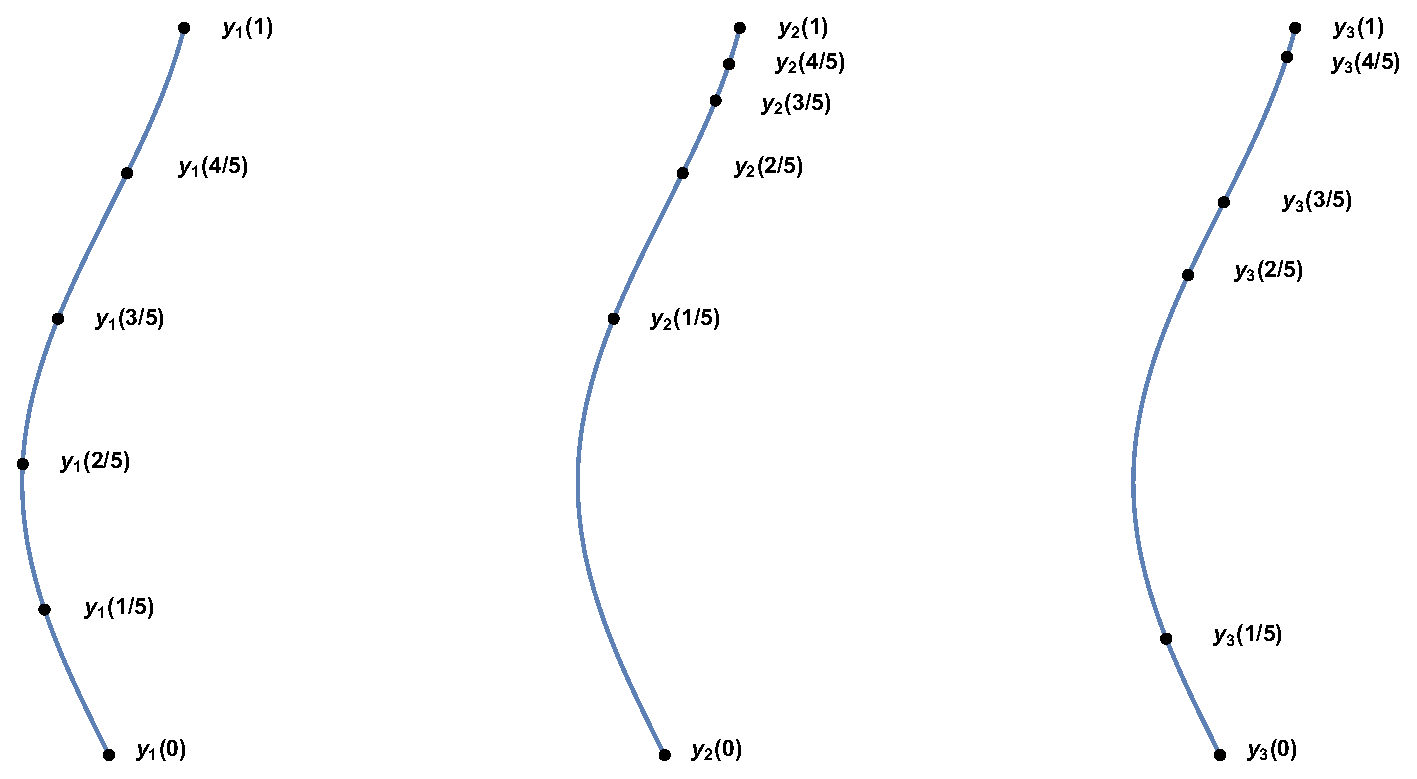
\includegraphics[height=0.6\paperheight]{curves.eps}
\caption{Różne parametryzacje krzywej $y$.}
\end{wrapfigure}
gdzie ma sens)
jest dyfeomorfizmem klasy $C^k$ (homeomorfizm z 
ciągłymi pochodnymi stopnia $k$). 
Zbiór $A$ map
 parami zgodnych (o zgodności klasy $C^k$) 
takich, że pokrywają cały zbiór $M$ nazywamy 
atlasem klasy $C^k$. Atlasem maksymalnym nazywamy atlas do którego
nie można dodać kolejnej mapy bez złamania zgodności.
Rozmaitością różniczkową klasy $C^k$ nazywamy 
zbiór $M$ z atlasem maksymalnym klasy $C^k$.
Wymiarem rozmaitości nazywamy wymiar przestrzeni $R^n$, na której 
modelujemy rozmaitość. Od teraz przyjmujemy, że rozmaitość 
jest klasy $C^\infty$ oraz $n=4$.
Rozmaitość nazywamy Lorenzowską jeśli określony na niej tensor
metryczny $g$ ma sygnaturę $(+,-,\dots ,-)$.

Będziemy stosować konwencję sumacyjną Einsteina. Ustalamy, że 
indeksy oznaczane literami greckimi zmieniają się w zakresie od 0 do 3, 
natomiast indeksy oznaczane literami arabskimi 
w zakresie od 1 do 3. Jednostki ustalamy tak, że $c=1$.
\subsection{Krzywe w czasoprzestrzeni.}
W tej części wprowadzimy pojęcie krzywej w czasoprzestrzeni. 
Jest to bardzo ważny obiekt matematyczny, gdyż służy do definiowania
wektora stycznego na rozmaitości różniczkowej~\cite{ganca1987}. 
%Większość ówczesnej fizyki formuuje się w postaci wariacyjnej,
%gdzie całkowanie odbywa się po pewnej krzywej.
\begin{definition}
Krzywą sparametryzowaną (lub parametryzacją krzywej) nazywamy 
odwzorowanie 
% gładki homeomorfizm
% homeomorfizm
$ y_1 : I \ni \tau \to y_1(\tau) \in M$ klasy $C^\infty$, 
gdzie $I \subset R$ 
jest przedziałem otwartym (niekoniecznie skończonym).
\end{definition}
\begin{definition}
Parametrem krzywej sparametryzowanej $y_1$ 
nazywamy funkcję $\tau_1$ taką, że $ y_1(I) \ni p 
\to \tau_1(p) = y_1^{-1}( p )\in I$. 
Będziemy pisać
$\tau_1$ zamiast $\tau_1(p)$, wszędzie gdzie punkt~$p$ 
wynika z kontekstu.
\end{definition}
\begin{definition}
Niech $y_1: I \to M$ i $y_2:J\to M$ będą parametryzacjami.
Reparametryzacją krzywej będziemy nazywać dyfeomorfizm $f : I \to J$
klasy $C^\infty$
taki, że $y_1 = y_2 \circ f$.
\end{definition}
Jeśli dla dwóch parametryzacji istnieje reparametryzacja to 
mówimy, że są one równoważne. Można łatwo pokazać, że jest to
relacja równoważności. Możliwość różnego parametryzowania tej 
samej krzywej możemy rozumieć tak, że możemy podróżować wzdłuż
krzywej w różny sposób.
\begin{definition}
Krzywą (lub krzywą niesparametryzowaną) nazywamy klasę równoważności
parametryzacji ze względu na powyższą relację równoważności.
Jeżeli $y$ jest krzywą, $y_1$ jej parametryzacją z parametrem $\tau_1$
to wprowadzamy oznaczenie $y_1 := y(\tau_1)$.
\end{definition}
\begin{definition}
Niech $(U,\ \xi)$ będzie mapą punktu$p\in U \subset M$. W tej mapie 
przez $y^\mu$ oznaczamy współrzędne krzywej~$y$.
Wektorem stycznym do krzywej $y$ w punkcie $p$  
(lub wektorem prędkości w 
parametrze $\tau$) nazywamy wektor $y'(\tau)$ taki, że
\begin{align*}
y' (\tau )= \frac{\d y^\mu (\tau) }{\d \tau}.
\end{align*}
Mając mapę w punkcie $p$ możemy określić bazę w danym punkcie
za pomocą wektorów stycznych do linii układu współrzędnych.
Taką bazę należy rozumieć jako bazę lokalną (bazę w punkcie $p$).
W bazie ortonormalnej macierz tensora metrycznego
przybiera postać 
\begin{align*}
( g_{\mu\nu} ) = \left(
\begin{array}{cccc}
1 & 0 & 0 & 0\\
0 & -1 & 0 & 0 \\
0 & 0 & -1 & 0 \\
0 & 0 & 0 & -1 
\end{array}
\right).
\end{align*}
Tensor metryczny $g$ wprowadza następujący podział wektorów:
\begin{align*}
g_{\mu\nu}u^\mu u^\nu > 0& \implies u \text{ - wektor czasowy,}\\
g_{\mu\nu}u^\mu u^\nu = 0& \implies u \text{ - wektor zerowy,}\\
g_{\mu\nu}u^\mu u^\nu < 0& \implies u \text{ - wektor przestrzenny.}
\end{align*}
\end{definition}
Powyższy podział wyróżnia trzy rodzaje krzywych: czasową, 
zerową i przestrzenną.
\begin{definition}
Krzywą $y$ nazywamy krzywą czasową (zerową, przestrzenną),
jeżeli w każdym punkcie $p \in y$ wektor~$y'$ jest 
wektorem czasowym
(zerowym, przestrzennym). Linią świata cząstki
jest krzywa czasowa lub, dla cząstek 
poruszających się z prędkością światła, 
krzywa zerowa.
\end{definition}
Długość $S(y(\tau))$ krzywej czasowej $y$ liczymy 
korzystając z tensora metrycznego $g$. 
Kwadrat długości elementu liniowego wyraża się przez
\begin{align*}
\d s^2 = g_{\mu\nu} \d x^\mu \d x^\nu.
\end{align*}
Stąd długość krzywej liczymy wzorem
\begin{align}\label{dlugosc_krzywej}
S( y(\tau) ) = \int_{\tau(p_0)}^{\tau(p_1)} \sqrt{g (
y' (\tau), y' (\tau) )} \d \tau.
\end{align}
Oczywiście 
długość krzywej nie powinna zależeć od wyboru parametryzacji.
Istotnie, długość dana wzorem~\eqref{dlugosc_krzywej}
jest niezmiennicza ze względu na reparametryzację.
Niech $\tau_1,\ \tau_2$ będą parametrami powiązanymi 
reparametryzacją  $\tau_2$~$=$~$f(\tau_1)$, taką że 
$f'(\tau_1) > 0$ (gdy $f'(\tau_1) <0$ rozumowanie 
przebiega analogicznie).
Stosując zmianę zmiennych całkowania dostajemy
\begin{align*}
S(y(\tau_2)) &= 
\int_{\tau_2(p_0)}^{\tau_2(p_1)} \sqrt{g (
y' (\tau_2), y' (\tau_2) )} \d \tau_2  = 
\int_{\tau_1(p_0)}^{\tau_1(p_1)} \sqrt{g \left(
\frac{ y' (\tau_1) }{ f'(\tau_1)}, 
\frac{ y' (\tau_1) }{ f'(\tau_1)} \right)} 
f'(\tau_1) \d \tau_1 = \\
& = 
\int_{\tau_1(p_0)}^{\tau_1(p_1)} \sqrt{g (
y' (\tau_1), y' (\tau_1)  )} \d \tau_1  
=S(y(\tau_1)).
\end{align*}
Stosując ten sam wzór do krzywej zerowej otrzymujemy zerową
długość. Od tej pory będziemy stosowali 
oznaczenie $ x\cdot y := g(x,y)$.

